%*****************************************
\chapter{A basic model for handwritten digits recognition}\label{ch:basic_tf_model}
%*****************************************

In this chapter we will discover a basic TensorFlow model developed in order to classify images from the MNIST dataset. Our scope is to illustrate the structure of a \acs{CNN} and how that basic model can be readjust as needed, gathering data about training accuracy during the epochs and test accuracy on known and unknown images from the dataset.

After an introduction to the MNIST dataset, we will study in deep the structure of the Convolutional Neural Network used in our experiments, trying to understand which parameters are relevant to the improvement of results, and how the structure can influence most of all on the accuracy of the network during training.

We identify two levels where we can intervene to modify the neural network. A architectural one, where we add, move and remove convolutional or pooling levels, and a parameter level, where we modify number of features, patch dimension, etc. The first one is more important, the second one is a more precise intervention.

\section{A focus on MNIST dataset}

Before beginning, let us focus on MNIST database, which is widely used in machine learning for training and testing. The acronym MNIST stands for Mixed National Institute of Standards and Technology because this database contains a large number of handwritten digits, it is a re-mixing of a previous dataset (NIST dataset) and collects $60000$ images for training and $10000$ for testing. The images were taken half from the American Census Bureau employees and half from American high school students and includes labels telling which digit it is.

\begin{figure}
	\centering
	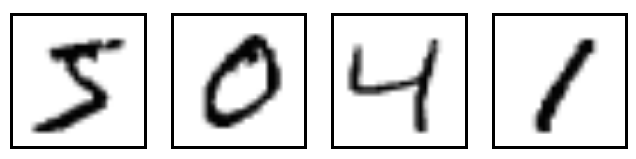
\includegraphics[width=0.7\textwidth]{Images/MNIST_images}
	\caption{Digit images from MNIST dataset}
	\label{fig:MNIST_images}
\end{figure}

Figure \ref{fig:MNIST_images} shows us four examples of handwritten digit images from MNIST dataset, in order we have 5, 0, 4, 1.

\subsection{Usage in the machine learning}

As mentioned earlier, MNIST dataset is widely used for training and testing neural networks, because it is a reference dataset in machine learning. During the years, lots of solution in neural networks research trained and tested on this dataset. Sometimes exciting results led to stale that neural networks achieved "near-human performance" But first attempts obtained mediocre results: a linear classifier had a error rate from $12.0 \%$ to $7.6 \%$, which is really not satisfying for such a simple task.

Other solutions led to better results. Non-linear classifier drastically reduced error rate to $3.3 \%$, but more appreciable results were obtained with 2-layers ($784-800-10$) neural networks, error rate: $1.6 \%$, $0.7 \%$ with elastic distortion. Boosted stumps achieved an error rate of $0.87 \%$, support vector machines $0.56 \%$, K-nearest neighbors $0.52 \%$ and 6-layer deep neural network $0.35 \%$.

The best result have been achieved with \acsp{CNN}: different kinds of \acs{CNN} reached the lowest error rate, from $0.31 \%$ to $0.21 \%$. Although the problem is quite simple, it clear that this kind of neural network is more powerful than others.

\subsection{Technical informations about images}

The digits have been size-normalized and centered in a fixed-size image of $28x28$ pixels. The dataset includes labels for each image telling us which digit it is.

Originally NIST dataset contained black and white, bilevel images. As a result of anti-aliasing technique used in normalization algorithms, images now contain grey levels. Digits were centered by computing the center of mass of the pixels and properly translating them.

Images are not in a standard image format, the data is stored in a very simple format designed for storing vectors and multidimensional matrices Clearly labels values are 0 to 9, while pixel values are 0 to 255, 0 is white and means background, 255 is black and means foreground; pixels are organized row-wise. In TensorFlow we normalize 0 to 255 values in 0 to 1 range.

\begin{figure}
	\centering
	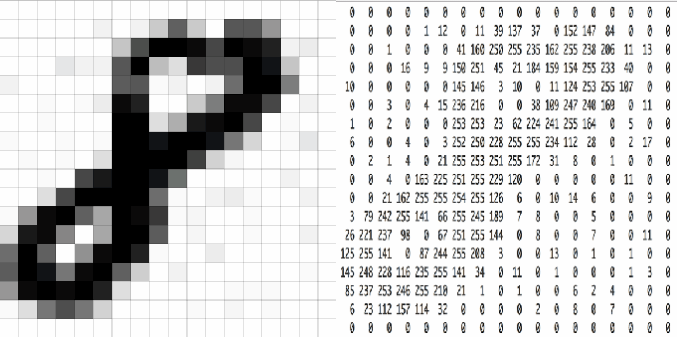
\includegraphics[width=0.9\textwidth]{Images/image_to_matrix}
	\caption{Example of translation from image to numeric matrix}
	\label{fig:image_to_matrix}
\end{figure}

Figure \ref{fig:image_to_matrix} shows uf an example of images storing format: each image can be translated in numeric matrix, pixel by pixel, encoding pixel colors (white, black and grey levels) in 0 to 255 range.

More detailed informations about data format are not useful to read and compute the files in the dataset.

\section{The hyperparameters level}

Editing hyperparameters of the network is very delicate, it is a precision intervention which hopefully allows uf to improve training and performance, or reduce in the worst case. We will consider the following parameters: number of features to identify in convolutional layers, patch size, stride size, number of input and output channels and padding of images.

\begin{description}
	
	\item[Number of features] That is one of the most important parameters to set, because here is specified how many features the network can learn. There is not a formula which allows us to find the perfect number of features based on the complexity of a task, but after several attempts with different values for this parameter we find a good solution for MNIST images. It can be concluded that a simple task, e.g. classify $28x28$ grey scale images of digits, requires a small amount of features: 8 in first convolutional layer, 16 in the second one. When we will analyze the result with different values of this parameter, we will find that extraordinary performance can be obtained with 2 and 4 features. Most difficult task with bigger and higher quality images, probably will require tens or hundreds features. An opposite problem is a too high value, the result is that some features can be equal or very similar, so it could be not really useful and performing.

	\item[Patch size] Patch size value allows us to adjust the size of the area where the network find features. Contrary to expectations, this parameter will not change from a convolutional and pooling layer to the next, because while it is a fixed value, the image dimension is reduced, so the patch cover a greater area and allows the recognition of more complex features in more space.  In our example with $28x28$ images a good patch size value is $5x5$. Obviously a bigger image require appropriate sized patch.
	
	\item[Stride size] According to the vanilla version proposed in the example, our stride value is 1. This value is combined with the padding in convolution ad pooling in order to obtain an input of the same size of the input.
	
	\item[Input and output channels] These parameters can vary from a convolutional layer to another. In the first layer the input channel is linked to the colors of the input images, so in our example we have the value 1; output channel value depends on the number of features recognized in the layer. In later layers the input channel must correspond to the output channel of previous layer, and output channel to the features recognized in the layer.
	
	\item[Padding dimension] As described previously with the formula, we determined the zero padding dimension. It is very important because with the stride size value permit to keep stable dimensions of input and output layer after layer.

\end{description}

\section{Main structure: the architectural level}

We introduced in Chapter 2 the different types of layers useful to build a \acs{CNN}], now we can analyze how they are combined in our TensorFlow model. This architecture was not modified, so it is exactly the one suggested in the TensorFlow example.

After the MNIST images are loaded, the TensorFlow session started and the variables initialized, we start building the multilayer \acs{CNN}.

\subsection{Weights initialization}

First of all we need to define a matrix of weights, its dimensions depend on images dimensions, so if images are $28x28$ pixel and we have $10$ categories, weights matrix have to be [$28*28$, $10$], so [$784$, $10$] dimensioned. At first weights are random values from a truncated normal distribution, the following code lines shows their initialization.

\begin{lstlisting}
def weight_variable(shape):
  initial = tf.truncated_normal(shape, stddev=0.1)
  return tf.Variable(initial)
\end{lstlisting}

\subsection{First convolutional layer}

The following code lines introduce the first block: a convolutional layer followed by the ReLU layer and the pooling layer. In the first two lines there is the initialization of weight and bias; weights are random values from a truncated normal distribution, bias is a constant tensor. Then on the third line there are convolution and ReLU operation, followed on the fourth line by the max pooling.

That kind of structure in the block we described is not the only solution, the different layers can be combined in different ways, e.g. we can add in this block a second convolutional layer instead of one before ReLU and max pooling.

\begin{lstlisting}
W_conv1 = weight_variable([5, 5, 1, features1])
b_conv1 = bias_variable([features1])
h_conv1 = tf.nn.relu(conv2d(x_image, W_conv1) + b_conv1)
h_pool1 = max_pool_2x2(h_conv1)
\end{lstlisting}

With Figure \ref{fig:conv_layer} we will help our reader to properly focus the structure of this layer, from the patches on the image which we can see in the figure, connected to the feature maps in convolutional layer, to the feature maps connected to the max pooling layer.

\begin{figure}
	\caption{A detailed schema of a convolutional and pooling layer with detailed notations}
	\label{fig:conv_layer}
	\centering
	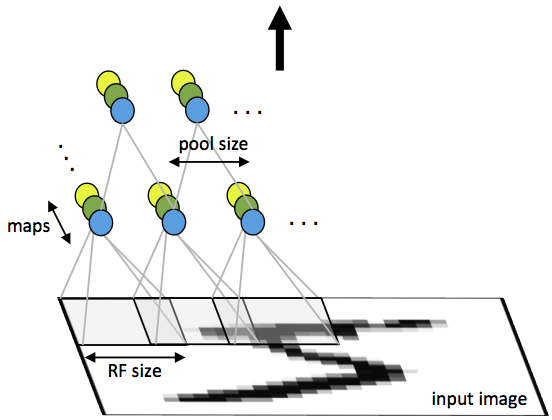
\includegraphics[width=1\textwidth]{Images/conv_layer}
\end{figure}

\subsection{Second convolutional layer}

Similarly to the previous subsection we can add a second block which has exactly the same structure of the first one: a convolutional layer with ReLU and pooling operations. The following code is equal to the previous, it does the same operations.

\begin{lstlisting}
W_conv2 = weight_variable([5, 5, features1, features2])
b_conv2 = bias_variable([features2])
h_conv2 = tf.nn.relu(conv2d(h_pool1, W_conv2) + b_conv2)
h_pool2 = max_pool_2x2(h_conv2)
\end{lstlisting}

The only difference between the two blocks we newly added is in the hyperparameters, in particular the number of features the network recognizes analyzing the images in input.

Any changes are possible: not only a single convolutional level con be added, but a whole block like the two we described right now. A more structured \acs{CNN} can be built with more complex task.

As we have so far tried to be clear and comprehensive describing this first part of the architecture in our basic model, we know it can be difficult to have figure the structure of all these levels. In order to help the reader, we provide Figure \ref{fig:conv_layers}.

\begin{figure}
	\caption{A schema of the two convolutional and pooling layers with detailed notations}
	\label{fig:conv_layers}
	\centering
	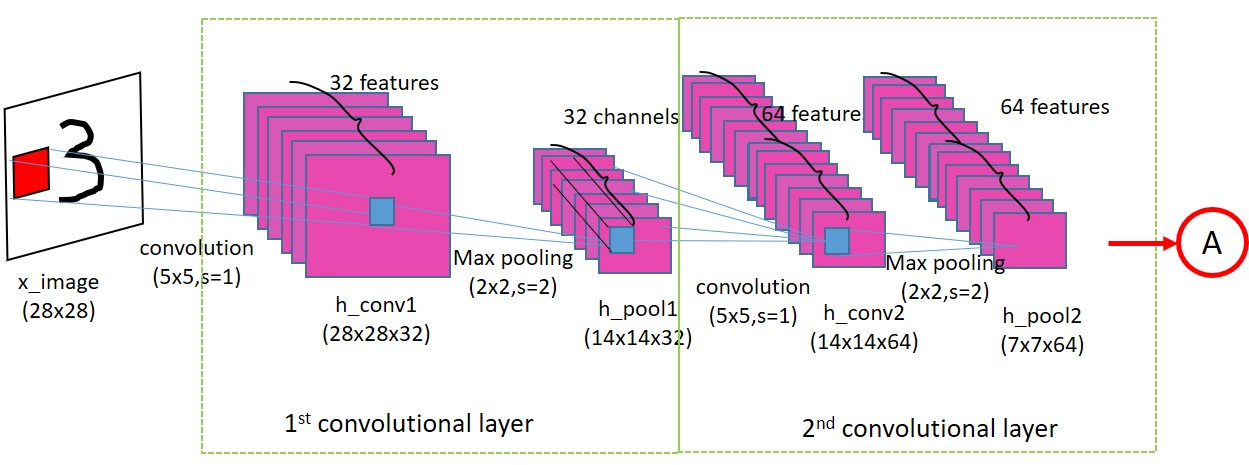
\includegraphics[width=1\textwidth]{Images/conv_layers}
\end{figure}

\subsection{Brief divagation on convolution and pooling function}

We introduced two convolutional layers, but we only saw the call of mask functions, both for convolution and pooling. Now we can have a little focus on these part in the code, so below we will find the respective functions.

The first, as can suggest its name conv2d, is the convolution function. Its parameters are:
\begin{itemize}
	\item[x] The 4d tensor, i.e. the images.
	\item[W] The weights matrix.
\end{itemize}

The masked call to a homonym function allows to specify also strides and padding.

\begin{lstlisting}
def conv2d(x, W):
	return tf.nn.conv2d(x, W, strides=[1, 1, 1, 1], padding='SAME')
\end{lstlisting}

Similarly, in pooling function, max pooling exactly, we have again x, strides and padding, which we already explained.

\begin{lstlisting}
def max_pool_2x2(x):
	return tf.nn.max_pool(x, ksize=[1, 2, 2, 1], strides=[1, 2, 2, 1], padding='SAME')
\end{lstlisting}

\subsection{Densely connected layer}

The densely connected layer is the core of classifying process in our \acs{CNN}, it is implemented as matrix multiplication added to a bias offset. With that layer it is also possible to learn combinations of features.

\begin{lstlisting}
W_fc1 = weight_variable([7 * 7 * features2, 1024])
b_fc1 = bias_variable([1024])
h_pool2_flat = tf.reshape(h_pool2, [-1, 7 * 7 * features2])
h_fc1 = tf.nn.relu(tf.matmul(h_pool2_flat, W_fc1) + b_fc1)
\end{lstlisting}

\subsection{Dropout layer}

In order to reduce overfitting we introduce a dropout layer, which is very important to perform better wih new examples. The implementation of that operations is really simple: a random set of activations is set to zero, so the pruned nodes are reinitialized and reinserted into the network. Dropout layer is used only during training, not during testing.

\begin{lstlisting}
keep_prob = tf.placeholder(tf.float32)
h_fc1_drop = tf.nn.dropout(h_fc1, keep_prob)
\end{lstlisting}

As we previously have done, we provide another image, Figure \ref{fig:other_layers}, to help the reader figuring the addiction of these new layers in the model architecture.

\begin{figure}
	\caption{A schema of the densely connected layer and dropout layer with detailed notations}
	\label{fig:other_layers}
	\centering
	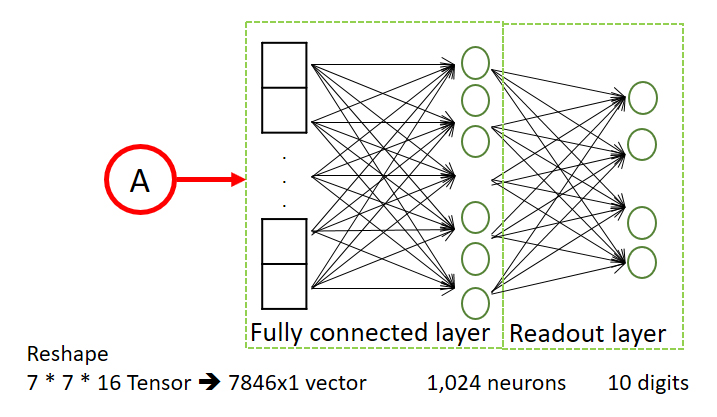
\includegraphics[width=1\textwidth]{Images/other_layers}
\end{figure}

\subsection{Loss (readout) layer}

The loss layer is the last one but also the core of regression model in our \acs{CNN}, here we find the implementation of regression model with the loss function: a multiplication of vectorized input images by the weight matrix, added to bias.

Our loss function is the cross entropy between the target and the softmax activation function applied to the model's prediction.

\begin{lstlisting}
W_fc2 = weight_variable([1024, 10])
b_fc2 = bias_variable([10])
y_conv = tf.nn.softmax(tf.matmul(h_fc1_drop, W_fc2) + b_fc2)
\end{lstlisting}

\subsection{Training, testing and evaluating the model}

\paragraph{Training}

We build our \acs{CNN} layer by layer, convolution by convolution and finally we defined the loss function. Now it is time to train that model and test its capabilities.

Train with TensorFlow allows to use automatic differentiation to find the gradient of the loss with respect to each of the variables. In the wide range of built-in optimization algorithms offered by TensorFlow we choose the Adam optimizer. The optimizer adds new operations, which include ones to compute gradients, compute parameter update steps, and applied update steps to the parameters.

\begin{lstlisting}
cross_entropy = tf.reduce_mean(-tf.reduce_sum(y_ * tf.log(y_conv), reduction_indices=[1]))
train_step = tf.train.AdamOptimizer(1e-4).minimize(cross_entropy)
correct_prediction = tf.equal(tf.argmax(y_conv, 1), tf.argmax(y_, 1))
accuracy = tf.reduce_mean(tf.cast(correct_prediction, tf.float32))
\end{lstlisting}

Training the model can be therefore be accomplished repeatedly running the train\_step for a number of epochs.

\paragraph{Testing and evaluating}

After a long training session, we want to evaluate performances of our network. It is possible with the following code line, where a percentage value of the accuracy is calculated.

\begin{lstlisting}
test_accuracy = accuracy.eval(feed_dict={x: mnist.test.images, y_: mnist.test.labels, keep_prob: 1.0})
\end{lstlisting}

Similarly we can evaluate the learning trend during training epochs. It is one of the most important measurement we made during lot of tests with different parametrized \acs{CNN}.

\section{Modifications of the architecture}

Previously we talk about architectural interventions, classifying them as more structural modifications. We reinvented the wheel during the first tests, where we tried to change something in the layers structure adding convolutional levels. Disastrous results led us to the conclusions that in case of quite simple task, like digits classification, ad excessive amount of layers ends in unsatisfactory results.

Just like the number of features should be assessed on the basis of task complexity, also the structure must be proportionate to it much more than hyperparameters.

Certainly task like facial recognition or high-defined images classification requires more complex structures, with more convolution levels and much more features.

\section{GUI for real time testing}

In order to have new experiences with our \acs{CNN} a simple \acs{GUI} was implemented. It allows us to test our trained network with real data not coming from MNIST dataset.

The \acs{GUI} uses a pre-trained network which detects $16$ and $32$ features in first and second convolutional layer. Users can draw digits with the mouse in a small box. The input is then processed in order to make it similar to images from the MNIST dataset. In particular the digit is rescaled in order to fit a $28x28$ pixel grid. Color values are normalized from $0$ to $255$ range to $0$ to $1$. $1$ represents a black pixel, while $0$ a white one.

The processed image is then mapped to a $28x28$ numeric matrix which is the input for the neural network. The digit corresponding to the input matrix is finally shown to the user. Figures \ref{fig:GUI_5} and \ref{fig:GUI_8} show two examples of digit recognition using the \acs{GUI}, in the first one the model recognize and correctly classify a $5$, in the second a $8$.

\begin{figure}
	\caption{Example of the GUI and the recognition of handwritten digit 5}
	\label{fig:GUI_5}
	\centering
	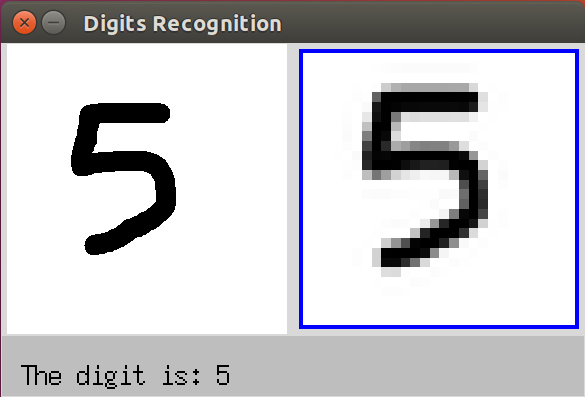
\includegraphics[width=0.8\textwidth]{Images/GUI_5}
\end{figure}

\begin{figure}
\caption{Example of the GUI and the recognition of handwritten digit 8}
\label{fig:GUI_8}
\centering
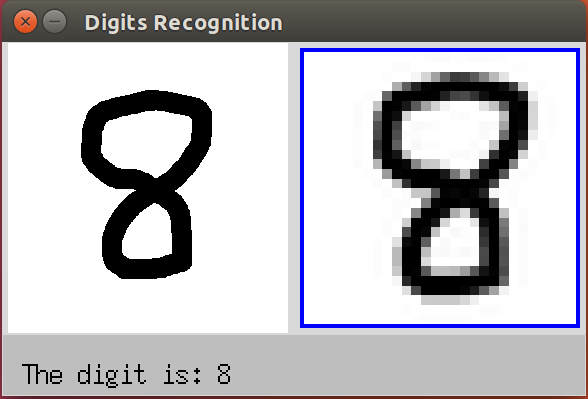
\includegraphics[width=0.8\textwidth]{Images/GUI_8}
\end{figure}